\chapter{Implementation}
\label{chap:2}

\section{Kubernetes Ready}
\begin{flushleft}
    Minikube is started by running \code{\$ minikube start}.\newline
    \subsection{API Containerization}
    As Kubernetes deploys containers as services, the Transactions API is first containerized.\newline
    The Transaction API container is built based on a Dockerfile found here \autocite{stevenDeployingDockerizedGolang2019} with some modifications. The reason for the
    two-step build is to keep the container size as small as possible. The API is built then the necessary files needed to run it are used in the final step.
    \begin{figure} [ht]
        \begin{center}
            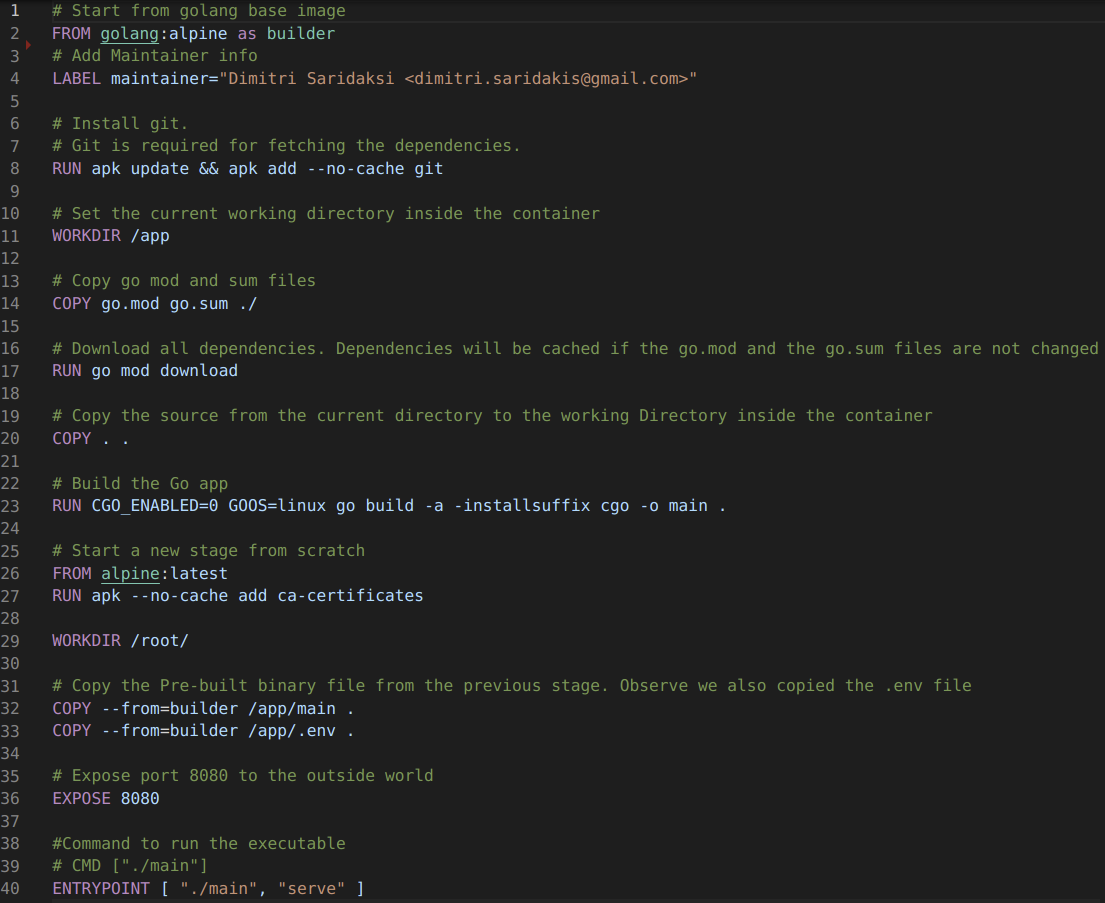
\includegraphics[width=.8\textwidth]{figures/apidockerfile.png}
            \caption{Transactions API Dockerfile}
            \label{fig: 2.1}
        \end{center}
    \end{figure}
    \pagebreak
    \newline There was a lot of testing carried out at this stage in perfecting the image and deploying both a PostGres container along with the API container.
    Most of the testing here was done using \code{docker-compose}.\newline
    In the API design, a custom logger was implemented, and its role was invaluable in debugging these steps from code to container to deployment.
    Every error/ important detail being documented from the exact line of code were the error/ event occurred along with the error/ event message/ details ensured that
    debugging was swift. Something else to note here is that the choice of GoLang for API design was a good one. In GoLang every error is treated
    as an error object and must be handled graciously to follow the Golang convention. This is not strictly enforced in the language as it is possible
    to just ignore the error object, but that has obviously negative effects on the application.
    \subsection{PostGres Containerization}
    This section was not trivial. By default, Debezium streams events in `pgoutput' format. A JSON format is the desired format so for this a `wal2json' plugin was downloaded.
    A new custom docker image had to be created which would specify the wal2json plugin to create a PostGres container which is capable of writing data to JSON format.
    \newline
    The Debezium connector specific components must also be included. As per the official documentation \autocite{LogicalDecodingOutput} There are two ways to do this.
    \bigbreak
    One is to install the components on a running PostGres database then containerize that database.
    \bigbreak
    Luckily, there is a far more straight forward method. The Debezium project has a repo on their GitHub \autocite{DockerimagesPostgres13} that makes this process easier with a dedicated build script.
    The repo was forked and git cloned locally. Then the build script was run as per \emph{Fig. 2.2}.
    \begin{figure} [ht]
        \begin{center}
            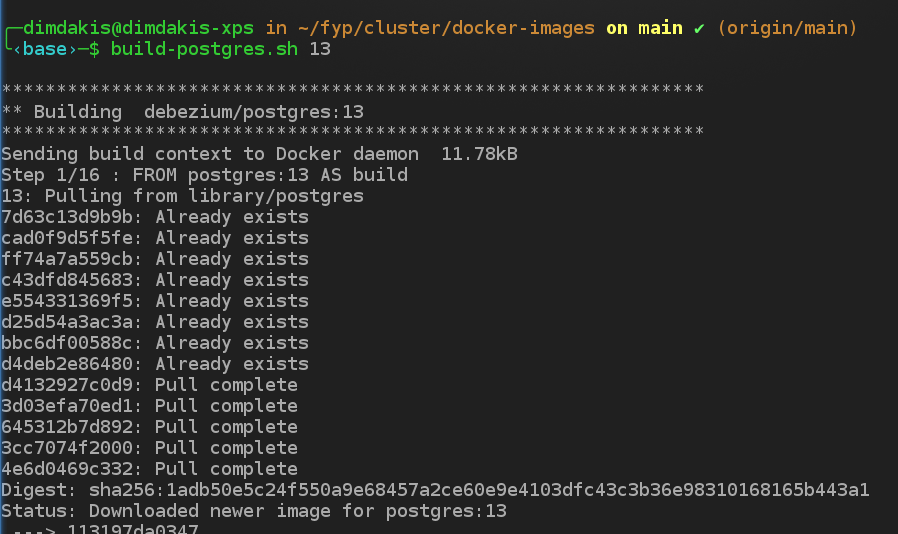
\includegraphics[width=1\textwidth]{figures/building-of-debezigres-image.png}
            \caption{Running the build script to generate the new Debezium friendly PostGres docker image}
            \label{fig: 2.2}
        \end{center}
    \end{figure}
    \bigbreak
    Whilst the build script did the job it was intended to do it saved the image as ``debezium/postgres:\emph{tag-name}''. This is somewhat
    problematic as there is already an image with that name on docker/hub. To overcome this obstacle the image had to be re-tagged as per \emph{Fig. 2.3}. Not a lot of work, but the
    process could just be a tad bit more user-friendly.
    \begin{figure} [ht]
        \begin{center}
            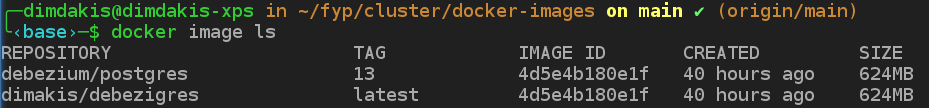
\includegraphics[width=1\textwidth]{figures/debezigres-tag.png}
            \caption{The initial and re-tagged PostGres friendly image.}
            \label{fig: 2.3}
        \end{center}
    \end{figure}

    \section{Deployment}
    Deployments in Kubernetes are made up of one or more identical replicas of a containerized application, as specified in the deployment manifest. Once a deployment is
    applied to the cluster. The Kubernetes Deployment Controller will automatically create the required number of replicas along with making sure that if any pods go down or
    become unresponsive new instances will be spun up in their place.\newline
    A Kubernetes Pod is simply a collection of containers that are run on a single node. Each pod can be thought of as a running process in the Kubernetes environment \autocite{PodKubernetesEngine}.
    Each container in a pod can share networking and storage resources with other containers in the same pod.
    \bigbreak
    Deployment of the system to Kubernetes must be done in a non-arbitrary order as some services depend on others. If the steps are done in the wrong order then the pods
    may get stuck in a \code{CrashLoopBackOff} state.
    \subsection{Automated Deployment}
    To simplify the deployment process, the initial section of deployment is farmed out to a Makefile. The Makefile is a simple shell script that runs the necessary commands to
    deploy the PostGres database container and then the API along with the required Kubernetes resources. It is simply run using \code{\$ make deploy}: \newline
    \begin{figure} [ht]
        \begin{center}
            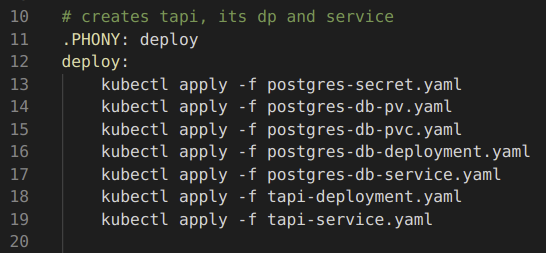
\includegraphics[width=.8\textwidth]{figures/deployment-makefile.png}
            \caption{The deployment Makefile}
            \label{fig: 2.4}
        \end{center}
    \end{figure}
    \pagebreak
    \subsection{Kubernetes Secret Object For PostGres and API}
    The first resource that is created is a Kubernetes Secret object. A Kubernetes Secret object is a file that contains sensitive information such as password, tokens, private
    IP addresses/ URLs, keys or any other data that the engineer chooses to hide from the application \autocite{Secrets} as per \emph{Fig. 2.5}.
    \begin{figure} [ht]
        \begin{center}
            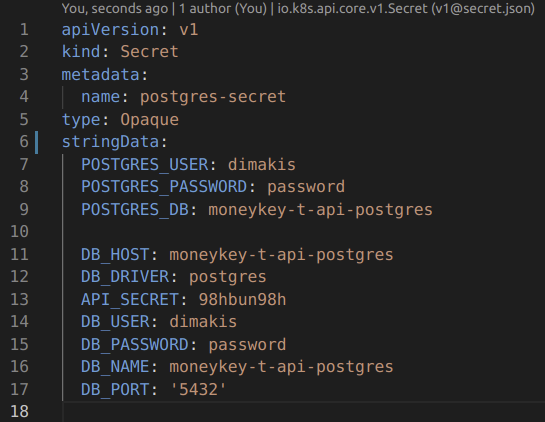
\includegraphics[width=.6\textwidth]{figures/deployment-secret.png}
            \caption{The Kubernetes Secret resource to be applied to the cluster with the real values altered.}
            \label{fig: 2.5}

            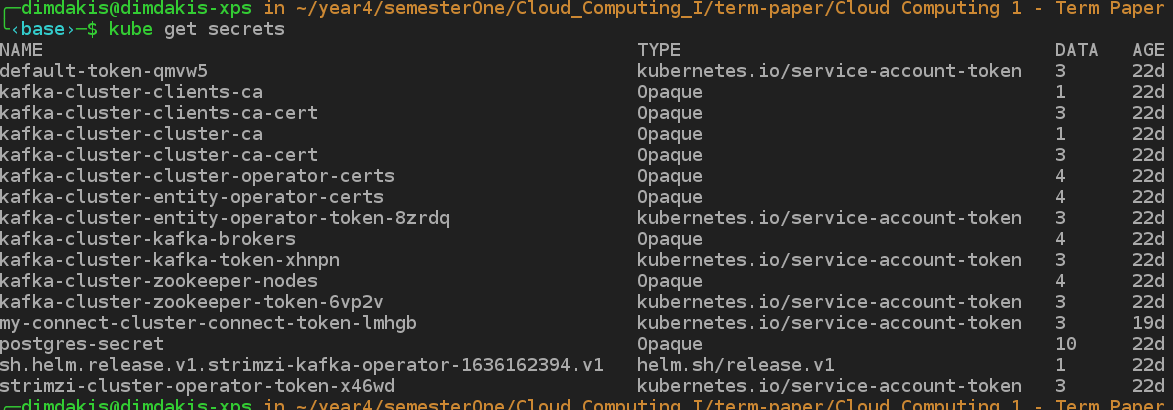
\includegraphics[width=1\textwidth]{figures/kube-get-secrets.png}
            \caption{Kubectl showing the secrets available in the cluster. \newline \textbf{Note:} The secrets of type `Opaque' are user defined secrets. Also note that on this
                system \code{kubectl} has long been aliased to \code{kube}.}
            \label{fig: 2.6}
        \end{center}
    \end{figure}
    \newline The secret values are then used to fill the environmental variables(ENV vars) in the API container.
    \bigbreak
    \subsection{PostGres Persistent Volume(PV)}
    The next resource object that is created is a Kubernetes Persistent Volume. A Kubernetes Persistent Volume is a storage resource that is backed by a file system. It allows for the
    application to store data in a persistent manner even though each instance of the application is ephemeral. \newline
    \begin{figure} [ht]
        \begin{center}
            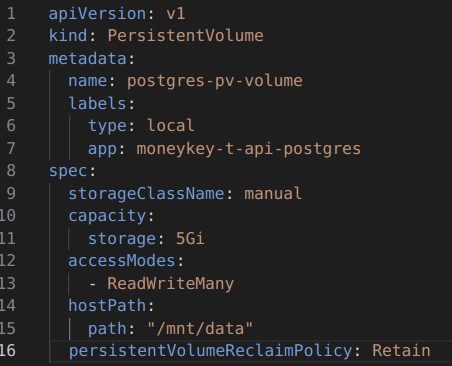
\includegraphics[width=.4\textwidth]{figures/postgres-pv.png}
            \caption{Manifest provisioning a persistent volume of size 5 GB which will be used for the PostGres database.}
            \label{fig: 2.7}
        \end{center}
    \end{figure}
    \subsection{PostGres Persistent Volume Claim(PVC)}
    The next resource that is created is a Kubernetes Persistent Volume Claim. A Kubernetes Persistent Volume Claim is a request for an existing Persistent Volume to be used
    with an application. The previously provisioned Persistent Volume is then bound to the Persistent Volume Claim for use with the PostGres database. \newline
    \begin{figure} [ht]
        \begin{center}
            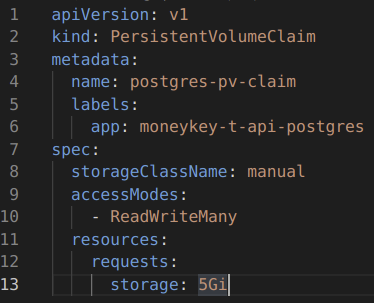
\includegraphics[width=.4\textwidth]{figures/postgres-pvc.png}
            \caption{Manifest binding the persistent volume to the PostGres database.}
            \label{fig: 2.8}
        \end{center}
    \end{figure}
    \pagebreak
    \subsection{PostGres Deployment}
    The next resource to be deployed is the PostGres deployment. In the deployment manifest the custom container image along with other required resources such as the secret from which
    the ENV vars should be populated, the persistent volume to be used and location to mount to along with the ports to be exposed are specified. \newline
    \begin{figure} [ht]
        \begin{center}
            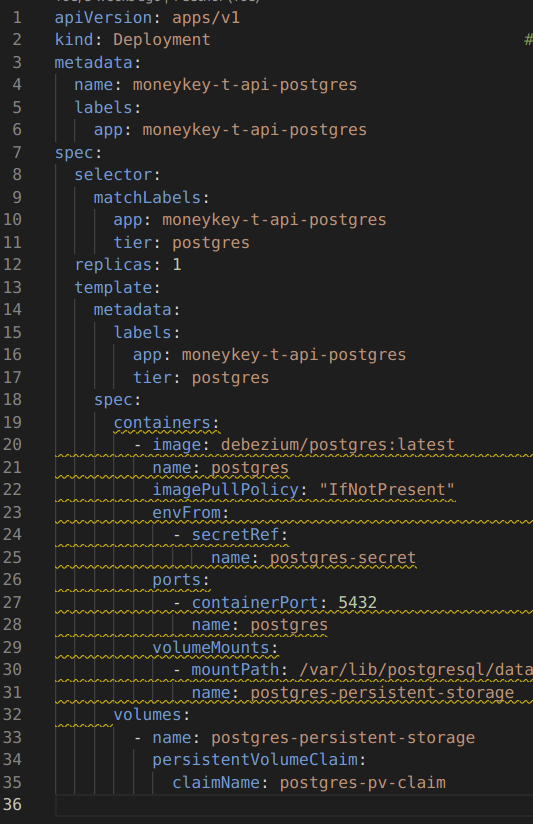
\includegraphics[width=.55\textwidth]{figures/postgres-deployment.png}
            \caption{PostGres deployment manifest. The yellow `warning' lines courtesy of VS Code, come from the Kubernetes extension. The warning is a result of not setting a
                resource limit on the deployment. As it is not yet known what kind of resources the deployment will require this warning will be ignored.}
            \label{fig: 2.9}
        \end{center}
    \end{figure}
    \pagebreak
    \subsection{PostGres Service}
    The last step to enable the database to run nominally is the service. A `service' object is the medium through which pods communicate with other pods in the system.
    Without exposing a service the database will not be accessible. \newline
    \begin{figure} [ht]
        \begin{center}
            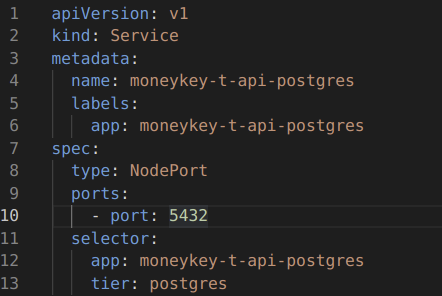
\includegraphics[width=.6\textwidth]{figures/pastgres-service.png}
            \caption{PostGres service manifest.}
            \label{fig: 2.10}
        \end{center}
    \end{figure}
    \subsection{API Deployment}
    The API deployment is a simpler process. It only needs a deployment manifest along with a service manifest. These are very similar to the PostGres versions as detailed above,
    save for application specific differences and as a result they will not be documented, however it is available in the `Supporting Material' section.
    \pagebreak
    \subsection{Test Deployment Thus Far}
    A simple test to determine if communication is possible between the API and the database, is to get the logs from the API container. As migrations are handled in the API,
    if these migrations appear in the logs then the system is nominal thus far:
    \begin{figure} [ht]
        \begin{center}
            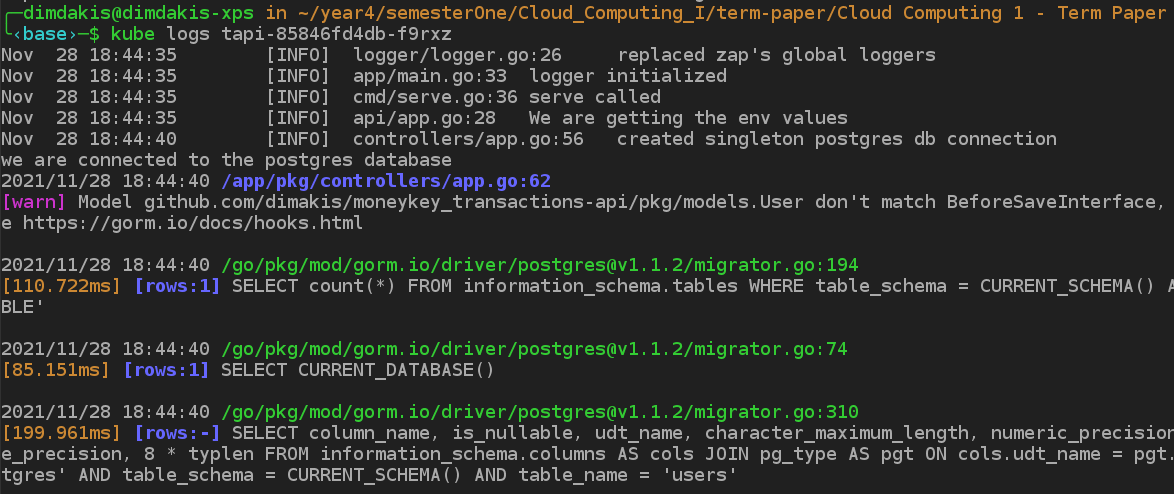
\includegraphics[width=1\textwidth]{figures/tapi-logs.png}
            \caption{Logs for the API container displays migrations to the database. This shows the two containers are communicating and behaving nominally.}
            \label{fig: 2.11}
        \end{center}
    \end{figure}
    \subsection{Strimzi Deployment}
    Kubernetes package manager Helm is used to deploy the Strimzi operator. Once Strimzi is deployed it will deploy a Kafka Broker, the Kafka Cluster Entity Operator and Apache Zookeeper.
    It is simply deployed using this command \code{helm install strimzi/strimzi-kafka-operator -n default} where the \code{-n} flag specifies the namespace to deploy to.
    \begin{figure} [ht]
        \begin{center}
            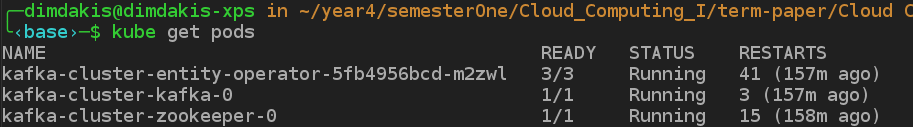
\includegraphics[width=1\textwidth]{figures/strimzi-deployed-kafka-componets.png}
            \caption{Helm successfully deploys the Strimzi Kafka Operator which in turn deploys the Kafka components.}
            \label{fig: 2.12}
        \end{center}
    \end{figure}
    \subsection{Kafka Connect for Debezium}
    The final installation and configurations are for Kafka Connect and the Debezium PostGres Connector. The first step is to create a Kafka Connect \emph{Custom Resource}(CR)
    Kubernetes object. This is done by applying the Kafka Connect \emph{Custom Resource Definition}(CRD) to the cluster.
    \begin{figure} [ht]
        \begin{center}
            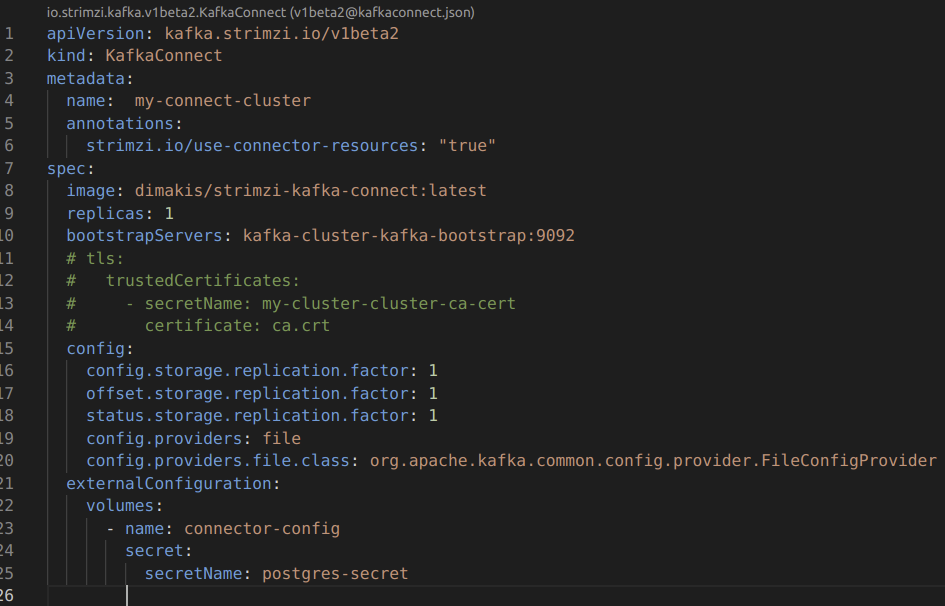
\includegraphics[width=1\textwidth]{figures/kafka-connect-manifest.png}
            \caption{Kafka Connect Custom Resource Definition manifest.}
            \label{fig: 2.13}
        \end{center}
    \end{figure}
    \newline \textbf{Note:} In the metadata the:
    \begin{lstlisting}
        annotations:
            strimzi.io/use-connector-resources: "true"
    \end{lstlisting}
    This allows for the Strimzi operator to automatically create the Kafka Connect resources based on this CRD.\newline
    Furthermore, a custom image is used. There were only minor changes from the default to suit this use case. \newline
    The traffic throughout the system is unencrypted. This would be a security concern in a production environment, however, for the sake of the time needed to
    add TLS the benefit didn't out weight the time outlay. In particular with the time spent on the configuration, testing and debugging of the system.\newline
    The \code{postgres-secret} is used here for the Kafka Connect cluster to connect to the PostGres database as without credentials it will not be authorised to connect.
    \subsection{Debezium PostGres Connector Deployment}
    The last step is to create the Debezium Connector. This is done by applying the Debezium Connector \emph{Custom Resource Definition}(CRD) to the cluster.
    \begin{figure} [ht]
        \begin{center}
            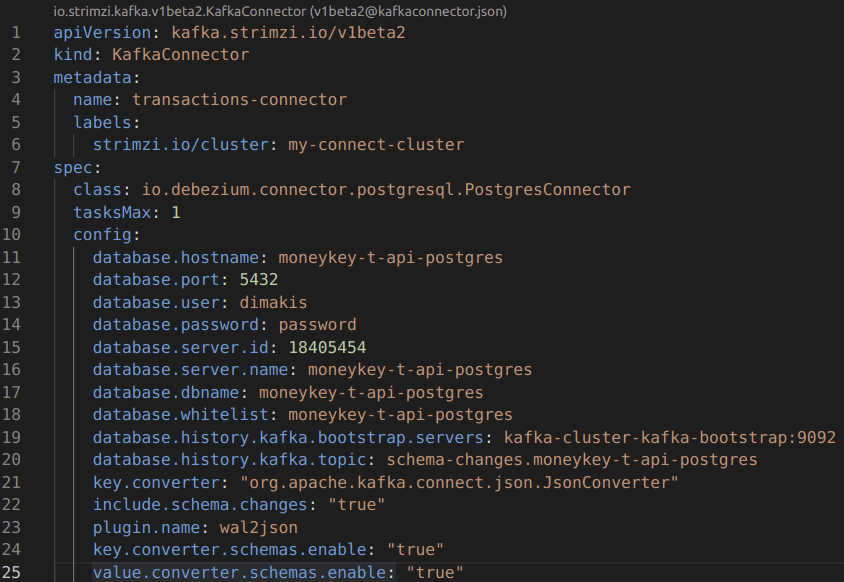
\includegraphics[width=1\textwidth]{figures/debezium-connector-manifest.png}
            \caption{Debezium PostGres Connector definition manifest.}
            \label{fig: 2.14}
        \end{center}
    \end{figure}
    \newline In this manifest the \code{labels} and \code{spec} are particularly important.\newline The \code{my-connect-cluster} label refers to the name given to the Kafka Connect cluster.
    This is what binds the Debezium connector to the Kafka Connect cluster. \newline The \code{config:} fields must match both the PostGres database details along
    with the appropriate Kafka configurations.
    \section{Testing the System}
    There are a number of ways to test the setup to see if everything is operational as intended. The first and quickest is to use \code{\$ kube get strimzi}.
    This should return all Kafka topics and other data about offsets etc.
    \begin{figure} [ht]
        \begin{center}
            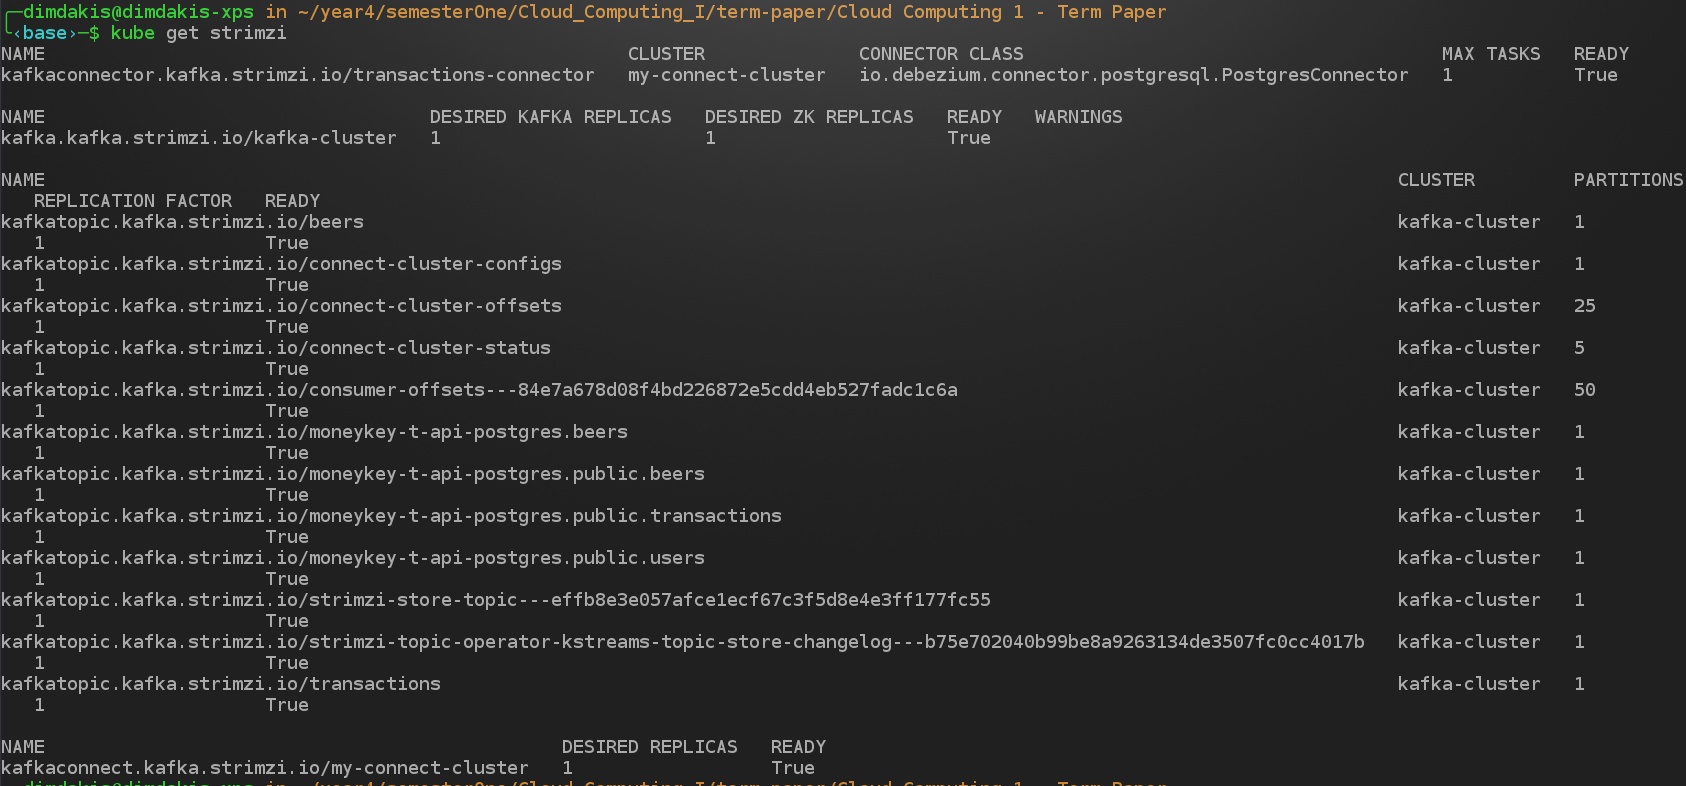
\includegraphics[width=1\textwidth]{figures/kube-get-strimzi.png}
            \caption{Kafka cluster information managed by the Kafka Entity Operator. This is the operator that manages both topics and users and the operator itself is
                deployed and managed by the Strimzi operator.}
            \label{fig: 2.15}
        \end{center}
    \end{figure}
    \newline As can be seen from \emph{Fig. 2.15} above, topics have been created with \code{..some code.. pulic.beers}, \code{..some code.. pulic.transactions} and
    \code{..some code.. pulic.users}. These are the table names from the PostGres database. It seems at very least the schemas have been created properly.
    \bigbreak
    To test the system in a live way, a simple Kafka consumer is created subscribing to one of these topics. The API endpoint will be exposed to external
    traffic(external to the Kubernetes cluster). Once this endpoint is hit, the data should be saved to the database where it will progress through the system and
    be observable via the consumer. The consumer is based on test image made available for this exact purpose via the Strimzi documentation hosted on Quay.io.
    This is the command to create the consumer:
    \begin{lstlisting}
        kubectl run kafka-consumer -ti --image=quay.io/strimzi/kafka:0.26.0-kafka-3.0.0 --rm=true 
            --restart=Never -- bin/kafka-console-consumer.sh 
            --bootstrap-server kafka-cluster-kafka-bootstrap:9092 
            --topic moneykey-t-api-postgres.public.beers
    \end{lstlisting}
    The image is pulled, Kubectl starts a new container from the image, once it is quit it will be removed. It connects to the Kafka Broker and the topic is the beers
    topic which comes from the \code{beers} table in the PostGres database.
    \bigbreak
    Minikube allows for an easy way to find the exposed API endpoint via the following command:
    \begin{figure} [ht]
        \begin{center}
            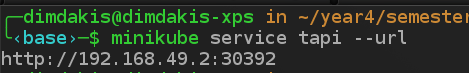
\includegraphics[width=.6\textwidth]{figures/minikube-service-url.png}
            \caption{The API's exposed URL via the service that was configured previously.}
            \label{fig: 2.16}
        \end{center}
    \end{figure}
    \bigbreak
    Postman is used to make a GET request to the service address and hit the \code{transactions/fake/create} endpoint. This will create a new transaction which we should
    be able to observe in both the response to postman and the terminal where the consumer is running. \newline
    Keep an eye out for the \code{beerName} value that is returned via the API response. It is a randomly generated beer name ``Ruination IPA''.
    \begin{figure} [ht]
        \begin{center}
            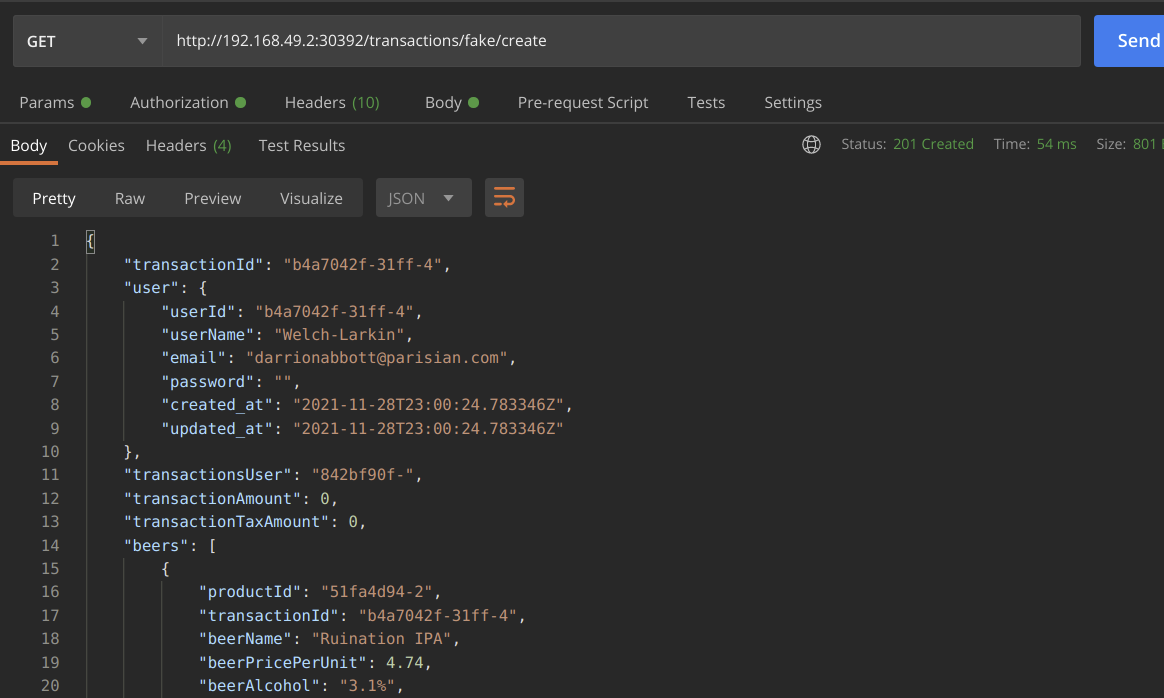
\includegraphics[width=1\textwidth]{figures/postman.png}
            \caption{Testing the endpoint with Postman. The response can be observed.}
            \label{fig: 2.17}
        \end{center}
    \end{figure}
    \pagebreak
    \newline As the response shows, a fake transaction is created. This proves that the API is accessible and that it does its job of creating some fake transaction data.\newline
    The final step is to check the output from the Kafka consumer:

    \begin{figure} [ht]
        \begin{center}
            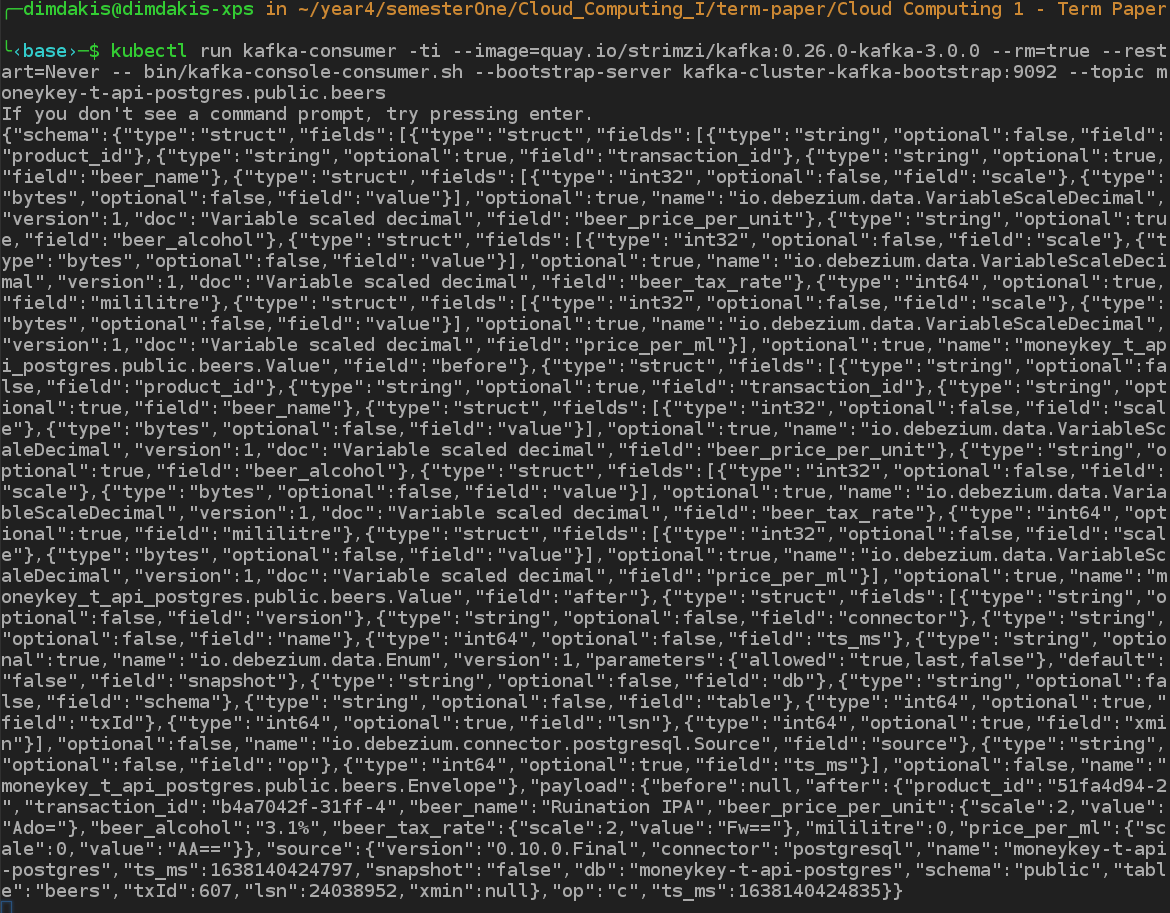
\includegraphics[width=1\textwidth]{figures/data-from-kafka-consumer.png}
            \caption{The data is streamed to the consumer via Debezium and the Kafka components.}
            \label{fig: 2.18}
        \end{center}
    \end{figure}
    Whilst there is a lot of output there, all schema and file type(GoLang structs that create the beer object) changes are being observed and recorded. This is configurable.
    If the same beer is in the output then we can be sure the system is working as intended. \newline

    \begin{figure} [ht]
        \begin{center}
            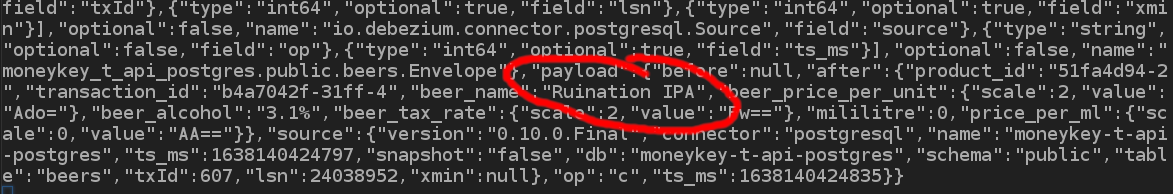
\includegraphics[width=1\textwidth]{figures/ruinationIPA.png}
            \caption{Proof of the newly created beer in the Kafka \code{beers} topic}
            \label{fig: 2.19}
        \end{center}
    \end{figure}
    \pagebreak
    Success! The system is working nominally, and that the data produced by the consumer is printed to the terminal instantaneously as the 
    GET request is made via Postman.
    \section{Challenges}
    There were very many challenges in the configuration of the system. At essentially every point along the way configuration changes had to be 
    implemented.
    \begin{itemize}
        \item The development of the Transaction API was a challenge.
        \item The creation of the PostGres container that is configured went through many iterations. Debezium requires certain configuration 
        to function. Replication permissions are required for a user, in this case a default user 1001, to be enabled. Replication logic itself
        must be set so that postgresql writes to the WAL in with a \code{logical\_decoding} setting \autocite{LogicalDecodingOutput}.
        \item Issues were had with docker-compose during the testing phase that required a purge of the docker-compose network. This wasn't a trivial
        fix either.
        \item The installation of Kafka via the Strimzi operator was a desperate last chance pivot. Initially Kafka was deployed via a custom 
        set of CRDs. However, there were very many connection issues and \code{CrashLoopBackOff} errors. The use of an operator was initially 
        thought to be too much to learn on top of the knowledge needed for the rest of the system. \newline However, the operator made it incredibly 
        easy (comparatively) to deploy the Kafka cluster.
        \item The deployment of Strimzi followed the same pattern as the Kafka deployment. Initially set up was using CRDs and the 
        use of Helm only stemmed from the goal of trying to automate the process. In doing so the installation of Strimzi became also much 
        easier and more automated.
        \item The largest chunk of time was probably spent on the configuration of the Kafka Connect cluster and the addition of the 
        Debezium Kafka Connector resource. The \code{kube  describe} command was used to check the status of the Kafka Connect clusters along 
        with CRDs whose deployment are automated via operators.\newline
        For quite a while a mere 1 value was left out of the configuration manifest. The seemingly obvious \code{database.server.name: moneykey-t-api-postgres}
        was omitted for far too long.
    \end{itemize}
\end{flushleft}